% !TEX root = ../../../main.tex
% 来源：中学数学实验教材·第二册（几何）
% 章节：直线形 / 三角形
% 原始文件：3.tex，行 1025-1031
% 类型：tikz
% ---
    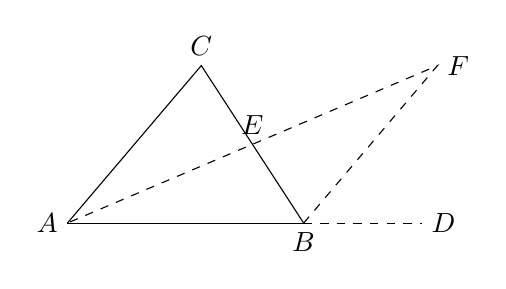
\begin{tikzpicture}[>=latex, scale=1]
\draw(0,0)node[left]{$A$}--(3,0)node[below]{$B$};
\draw[dashed](3,0)--(4.5,0)node[right]{$D$};
\draw(3,0)--(1.7,2)node[above]{$C$}--(0,0);
\draw[dashed](3,0)--(4.7,2)node[right]{$F$}--(0,0); 
\node at (2.35,1)[above]{$E$};
    \end{tikzpicture}
